\chapter{Literature Review}


% ------------------------------------------------------------ %


\section{Research Methodology}
\textcolor{red}{WIP}\\
In the methodology section, the we first delves into the existing literature, drawing from a paper accessible through the platform "Paper with Code." This platform typically provides research papers along with their associated code implementations. The chosen paper appears to be selected based on its prominence, likely measured by its reported accuracy or success in the field.
Following the identification of the primary paper, the researcher conducts a thorough review of its content, focusing particularly on aspects related to methodology. This involves understanding the proposed techniques, algorithms, and approaches presented in the paper to achieve high accuracy in the context of text-based person searches. The aim is to comprehend the nuances of the existing methodology and identify the key factors contributing to its success.
In addition to the primary paper, the researcher examines two other papers that exhibit a significant difference in accuracy. This comparative analysis is valuable for gaining insights into different approaches within the field. The choice of these additional papers may be strategic, aiming to capture diverse perspectives or methodologies, especially if there is a notable contrast in their reported accuracy metrics.
The researcher likely scrutinizes the methodologies of these selected papers, comparing and contrasting them with the primary paper. This comparative analysis helps identify the strengths and weaknesses of different approaches, shedding light on potential areas of improvement or innovation for the current research.
Overall, the methodology involves a comprehensive exploration of relevant literature, with a focus on the primary paper selected from "Paper with Code." The intent is to understand the methodologies employed in achieving high accuracies and to leverage insights from other papers with varying performance metrics. 

However, if only paperwithcode is used, the information obtained is limited and biased. To eliminate this bias, we decided to use scopus to search a wider range of papers by keyword search.

\subsection*{Identification}

The following research question was defined:

\bigskip
\textit{``Can lightweight models maintain detection accuracy in text-based person search?''}
\bigskip



From this research question, four main keywords that sufficiently explain the topic were used: person retrieval and vision language pre-training.
Furthermore, synonyms and related terms were associated to these keywords to form keyword groups as follows:

\begin{itemize}
    \item person retrieval:
    \begin{itemize}
        \item person;
        \item person detection;
        \item person search.
    \end{itemize}
    \item vision language pre-training:
    \begin{itemize}
        \item VLP;
        \item text based;
        \item text.
    \end{itemize}
\end{itemize}


From the keywords, we had a keyword search on scopus from the search strings as follows:

\begin{itemize}
    \item ( "person retrieval" OR "person" OR "person detection" OR "person search" ) AND ( "vision language pre-training" OR "VLP" OR "text based" OR "text" ).
\end{itemize}

The Scopus search yielded a total of $20170$ documents. Within this result, we set the subject area to Computer Science, document type to article and conference paper, language to only english, and set the open access to all open access. With this filters, $862$ articles were found. 

\subsection*{Screening}

Various factors were taken into account for the exclusion of documents:
\begin{enumerate}
    \item problem and goal were too different (e.g., building new hardware, analysis of leaf reflectance);
    \item not sufficiently related to this work (e.g., focused on hyperspectral );
    \item duplicates that were not automatically detected and excluded.
\end{enumerate}



% ------------------------------------------------------------ %

\section{Transformer}
\textcolor{red}{WIP}
% general explanation of transformer
% Transformer is an encoder-decoder model which is made with attention mechanism \cite{vaswani2023attention}. This model was first created to solve the problem of "lack of understanding the global nuances" and "faster training speed" which the Seq2Seq had. The author approach to this problem by applying a mechanism called "attention" to understand the caution expression. This is similar to gate mechanism in LSTM where they emphasizes the important information, and make unnecessary information inconspicuous. By this method, the model can focus to the important information from the enormous information to process. 

The Transformer model, introduced by Vaswani et al. \cite{vaswani2023attention}, is an encoder-decoder architecture featuring an attention mechanism. Initially devised to address the limitations of the Seq2Seq model, such as the challenges in grasping global nuances and the need for faster training, the Transformer model leverages attention mechanisms. These mechanisms, akin to the gating mechanism found in LSTM networks, prioritize important information while suppressing irrelevant details. By employing this approach, the model can effectively discern crucial information from the vast array of input data for processing.

Structure of the Transformer is shown figure\ref{fig:transformer}. The model is structured as encoder-decoder model, most competitive neural sequence transduction models are also encoder-decoder model, with encoder maps an input of symbol representation $X=(x_1, ...,x_n)$ toa continuous representation $Z=(z_1,...,z_n)$. The decoder will take the given z to generate an output sequence of $(y_1,...,y_n)$ of symbols one at a time.

\begin{figure}[htbp]
    \begin{center}
        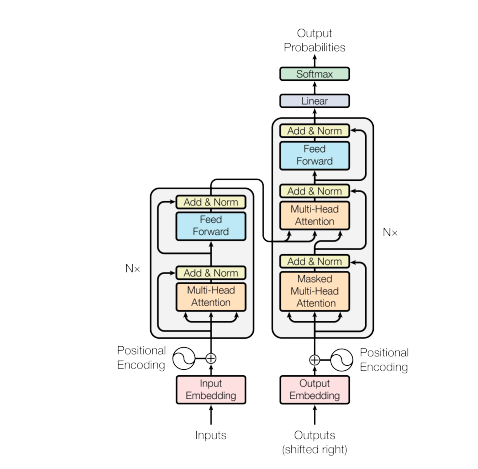
\includegraphics[width=10cm]{img/transformer.png}
        \caption{Structure of the Transformer}\label{fig:transformer}
    \end{center}
\end{figure}

% % talk about transformer block, plus multihead attention
% Transformer Block is the unit for transformer, and this contains multi-head attention and position wise feed-forward networks. Transformer block has three input Query, Key, and Value which is used for computing attention representation on Multi-head attention.
% The position-wise feed-forward networks converts the output of Multi-head Attention to for each tokens. Skip connection is placed between the layers to decrease the gradient loss, which enables deepening the model. 

% % image of transformer block with q,k,v input

% To explain Multi-Head attention, we first describe the Single-Head Attention. Single-head Attention is a Attention module with only one Scale-Dot Product. 

\section{Vision-language pre-training}
\textcolor{red}{WIP}

Vision and Language(VL) is a major research area for the causality of Computer Vision and Natural Language Processing (NLP), which aims to effectively learn from multimodal data. Some of the great success of language model pre-training in NLP(RoBERTa(\cite{liu2020roberta}), BERT(\cite{devlin2018bert}), and GPT-3(\cite{brown2020language})) influenced the field of Vision-Language Pre-training (VLP) to grow attention from both fields. 

The existing methods for VLP rely on object detection models, multiple auxiliary objectives, and limited-scale human annotation data. To solve this challenges, blah,blah,blah....

Current works in VLP fields we have is the 
VisualBERT
A joint representation model for VL task which is designed to capture rich semantics in the image and associated text. The author integrated BERT for the NLP task with pretrained object proposal systems like Faster-RCNN. Figure\ref{fig:visualvert} shows how the model is trained. 

\textcolor{red}{blah,blah, blah}
\begin{figure}[htbp]
    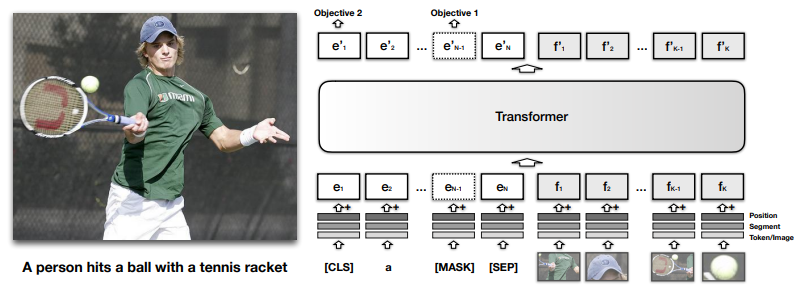
\includegraphics[width=10cm]{img/VisualBERT.png}
    \caption{Representation of VisualBERT}\label{fig:visualvert}
\end{figure}


SimVLM simple visual language model
Minimalist pretraining framework for joint visual and textual representation. The motivation for this research is the limitations and complexity of existing vision-language pretraining models, which often require expensive annotations and multiple dataset-specific objectives. SimVLM aims to address these issues by utilizing large-scale weak supervision and training end-to-end with a single prefix language modeling objective.


CLIP is build on a vision transformer architecture, similar to BERT but instead of joint representation model, CLIP uses different encoder for both modal and from the extracted features, we calculate the dot product. During the learning process, the diagonal component of this matrix are learned to have larger values than the others.

Recent studies shows that bigger the learning dataset, the better accuracies. 

\section{Person Understanding Task}
in this section we will talk about different method we can use for person understanding task. 

\subsection{Text-based re-identification}
\textcolor{red}{WIP}\\
This section presents papers that study text-based person retrieval. A common issue addressed in each paper is the deficiency of the feature from text and image encoders. It has been confirmed that when the features of each modal are integrated, information is distorted or missing, which affects the accuracy of detection. Therefore, how to resolve this deficiency is key in this section.

\subsubsection{RaSa: Relation and Sensitivity Aware e Representation Learning for Text-based Person Search}
\textcolor{red}{WIP}\\
This paper introduces a method called Relation and Sensitivity Aware representation learning (RaSa) that includes two novel tasks: Relation-Aware learning (RA) and Sensitivity-Aware learning (SA). It addresses the shortcomings of existing methods in text-based person search, where clustering representations of positive pairs without distinction leads to overfitting, particularly with weak positive pairs. RA mitigates overfitting by introducing a positive relation detection task to distinguish between strong and weak positive pairs. Additionally, the author emphasizes the common practice of learning invariant representation under data augmentation for robustness but goes further by encouraging the representation to perceive sensitive transformations through SA, promoting enhanced robustness by detecting replaced words in textual descriptions.

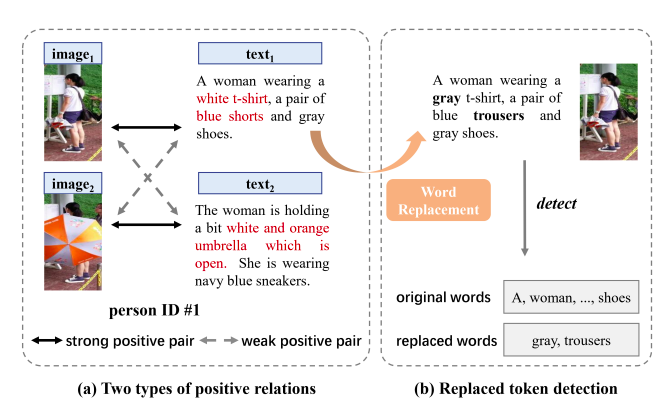
\includegraphics[width=10cm]{img/rasa.png}


\subsubsection{Cross-Modal Implicit Relation Reasoning and Aligning for Text-to-Image Person Retrieval}
The paper introduces a novel approach, called IRRA (Implicit Relation Reasoning and Aligning), for text-to-image person retrieval. This task i`nvolves identifying a person based on a given textual description. The main challenge is to establish an effective mapping between visual and textual modalities in a shared latent space. Unlike previous methods that use separately pre-trained unimodal models, IRRA addresses this challenge by introducing a cross-modal Implicit Relation Reasoning module. This module integrates visual cues into textual tokens through a masked language modeling paradigm, facilitating cross-modal interaction. To globally align visual and textual embeddings, the paper proposes Similarity Distribution Matching, which minimizes the KL divergence between image-text similarity distributions and normalized label matching distributions. 

\subsubsection{Learning Semantic-Aligned Feature Representation for Text-based Person Search}
The paper focuses on text-based person search, aiming to retrieve images of a specific pedestrian based on a textual description. The primary challenge in this task is to bridge the inter-modality gap and align features across textual and visual modalities. The proposed solution is a semantic-aligned embedding method that automatically learns feature alignment between visual and textual representations. The method utilizes two Transformer-based backbones to encode robust feature representations for images and texts. Additionally, a semantic-aligned feature aggregation network is introduced, incorporating a multi-head attention module constrained by a cross-modality part alignment loss and a diversity loss. 


% \subsection{Image-based re-identification}
% with the image based methods, we have the old fashion way of cnn 



\subsection{person attribute recognition}
person attribute recognition has seeked to have supervision 
... made a mask on the person to set the person 
... tried to slice the image so that we can extract specific parts from the person
... tried to create a filter 

% ------------------------------------------------------------ %
